%!TEX root = ../../../main.tex

\section{Coupling \SIVS to \Vcsels} \label{sec::coupling_vcsel}

	In the context of metrology, controllable \spss, operating at room temperature, are an extremely important prospect. Such devices are anticipated to play a key role in the development and calibration of detectors and measurement methods aiming to resolve optical flux down to single-photon resolution \cite{Vaigu2017}. As such \sps form a cornerstone of the efforts directed towards the redefinition of the candela in terms of single photons, see discussion in \Fref{ch::introduction}.

	Here we attempt to create a hybrid-integrated \sps by placing a \nd ideally containing a solitary \sivs on-top of a \vcsels (\VCSELs). Using \nds containing exactly one \sivs is a necessary requirement for the realization of a proper \sps, however, such \nds are difficult to identify. Thus, we rely on \nds containing several \sivs for a first poof-of-concept implementation demostrating the validity of coupling emmitters to \VCSELs.

	In our approach a \nd containing \sivs is situated such that output laser of the \VCSEL can be used to optically excite the \cc. Since the \VCSEL laser can be controlled very well, \siv operation can be steered reliably. Through the use of suitable optical filters allowing only \siv \fl to emerge, a controlled \sps can be realized in principle.

	In the following we give a short discussion of \VCSELs. Next we discuss the coupling of \sivs to \VCSELs and report on the optical properties of the resulting hybrid-integrated light source.

	\subsection{\Vcsels}\label{subsec::vcsel_structure}

		% britney = http://britneyspears.ac/physics/vcsels/vcsels.htm
		A \vcsel is a type of semi-conductor laser diode \cite{melngailis1965longitudinal, ibaraki1984pulsed}. \Fref{fig::vcsel_sketch} illustrates a common design consisting of a $p$-layer on top and a $n$-layer at the bottom separated by a so-called active area. When a current is applied across the device, charge carriers migrate towards the active region. Holes act as charge carriers in the $p$ region, whilst electrons carry charge in the $n$-region. The material properties of the active region is chosen such that when electrons and holes spontaneously recombine, a photon is emitted in the process. Electron-hole pairs can also dissipated via the creation of phonons leading to losses in the form of heat. To define the region for recombination to occur and to control the optical properties of the device, additional thin layers of semi-conducting material can be introduced in the active area. These result in the formation of quantum wells with associated energy levels and resulting preferred transitions with well-defined energies for the recombination of electrons and holes.

		\begin{figure}[!htb]
			\centering
			\testbox{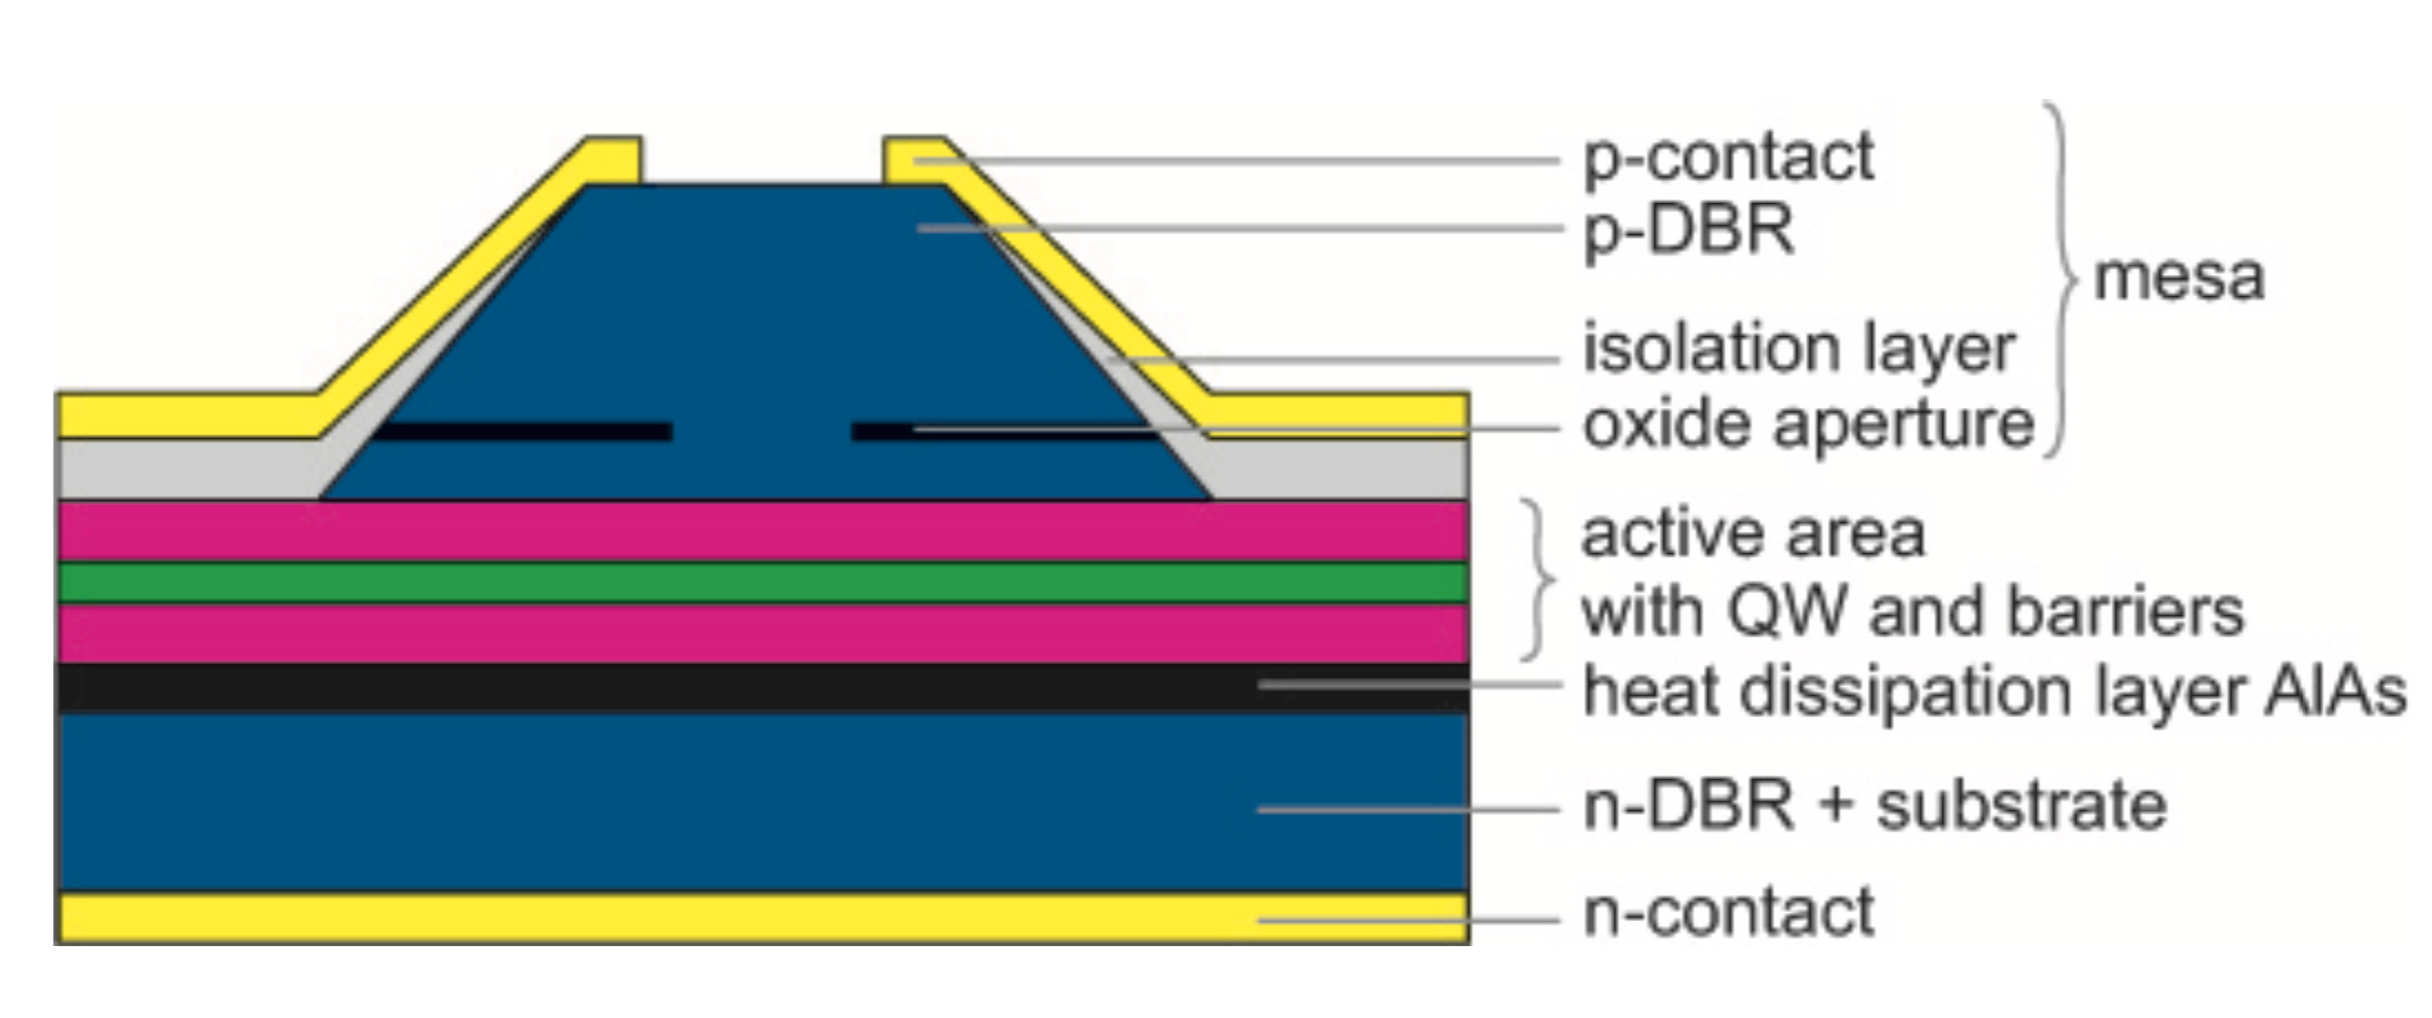
\includegraphics[trim = 0 0 0 0,  clip= true, width = \pairplotwide]{./pics/vcsel_sketch.png}}
			\caption[Sketch of a \vcsel]{Illustration of a \VCSEL laser diode \cite{Weidenfeld}. When a current is applied across the device via contacts (yellow), holes and electrons migrate from the $p$-region (blue, top) and the $n$-region (blue, bottom) towards the active region (purple+green, center) where they recombine emitting photons. A quantum well is inserted in the active region, shaping the recombination process. $p$-region and $n$-region are acting as DBRs forming the resonator of the laser. When enough photons are gained by via stimulated emission, a laser beam emerges from the $p$-region after passing an oxide aperture.}
			\label{fig::vcsel_sketch}
		\end{figure}

		To achieve lasing, stimulated recombination and thus stimulated emission of photons is required. To facilitate this both $p$-region and $n$-region are constructed in a layered fashion allowing them to act as highly-efficient distributed Bragg reflectors (DBR). Thus the active region is sandwiched by two mirrors forming the resonator of the laser diode. Spontaneously emitted photons thus are temporarily trapped continuously interacting with the active region. Provided the presence of sufficient electron-hole pairs, a photon can stimulate their recombination and thus the emission of further identical photons which themselves increase the stimulated emission. If enough identical photons are gained in this process, a coherent laser beam is formed by the fraction of photons escaping the resonator through the $p$-region. As a result the laster beam produced by a \VCSEL is perpendicular to the substrate it resided on.

		\VCSELs have a range of properties that make them particularity interesting for industrial applications such low power consumption, ease of fabrication and cheap production. As a result, \VCSELs are utilized in a broad range of applications including fiber optic communications or precision sensing and are used widely in commonly encountered devices such as computer mice or laser printers \cite{Weidenfeld}.

		In the context of this thesis \VCSELs offer several advantages. Their output beam is perpendicular to the substrate surface and suitable to excite \sivs. This means that \nds containing \sivs can simply be placed ontop of the device. Furthermore their physical size is ideal for the \nds we work with. The small size of \VCSELs will make it easier to deploy the resulting hybrid-integrated light sources in future applications.

	\subsection{\SIV in a \Vcsel}

	% Vertical-cavity surface-emitting lasers are attractive candidates for emerging technologies such as high-density optical storage systems, high-definition laser printing and optical communication systems using polymer optical fibers (POF). The red AlGaInP-based oxide-confined vertical-cavity surface-emitting lasers (VCSEL) target one absorption minimum of the polymer optical fibers (POF) at around 650 nm. In addition, VCSELs are compact, exhibit circular beam profile and have low divergence angle, in contrast to edge-emitting laser, for an easy coupling of light into the fiber. Furthermore, they offer high-speed modulation capability (several GHz) [1] which is required for optical data communication.
	% \\
	% The VCSEL structure (Fig. 2) consists of an laser active region embedded in between two distributed Bragg reflectors (DBR). For maximum modal gain the current and the optical mode need to be confined in the transverse direction for serving as a spatial filter. This is achieved with an implemented oxide aperture, with diameter DA, directly above the active region in a field node of the standing wave field to minimize scattering losses. Our devices possess optical output power up to 3 mW with low threshold current (1 mA) at 660 nm. For practical application a stable single transverse mode especially the fundamental mode and a stable polarization of the emission is desirable owing to higher coupling-efficiency into optical fibers.
	% \\
	% II. EXPERIMENTAL PROCEDURE The investigated VCSEL structures were grown by metalorganic vapor-phase epitaxy (MOVPE) in an AIX-200 hori- zontal reactor setup with in situ growth control using stan- dard sources at low pressure of 100 mbar and a tempera- ture of 750 ◦C on (100) n+-GaAs substrate misoriented 6 ◦ towards [111]A. The bottom n-type DBR is made of 50 pairs of AlAs/Al0.5Ga0.5As. The p-type DBR consists of 36 Al0.95Ga0.05As/Al0.5Ga0.5As mirror pairs. Four compres- sively strained GaInP quantum wells (QW) built up the active region. To realize an oxide aperture, the advantage of high oxidation selectivity of the AlxGa1−xAs material system is used. We use an Al-content of x = 0.98 for this oxidation layer. Active diameters DA from 3 µm to 20 µm were obtained on one sample because of the flow profile of the nitric water vapor in the oxidation chamber. To investigate the transverse beam profile depending on different parameters we built up a vertical measurement setup. The beam profile is mapped with a lens system of 3 lenses and captured with a CMOS-camera. The vertical setup provides the advantage of on-wafer-testing.

	To conduct our research, we received an array of red AlGaInP-based oxide-confined \VCSELs from \michler. The array includes three individually operable \VCSELs, two of which, labeled \BmFour and \BmTwo were used in our experiments, see \Fref{subfig::vcsel_sem_big_overview}.

	\begin{figure}[!htb]
		\begin{subfigure}[t]{ 0.49\linewidth}
			\centering
			\testbox{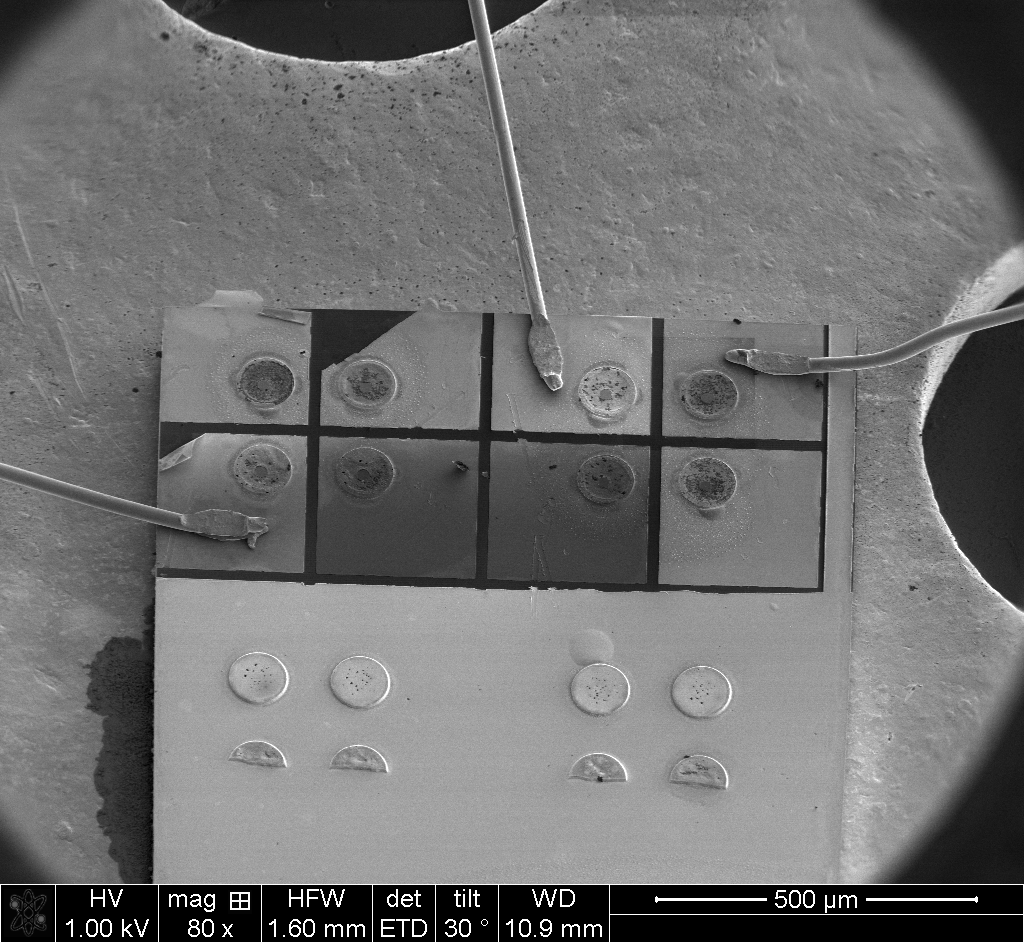
\includegraphics[trim = 0 0 0 0,  clip= true, width = \pairplotwide]{./pics/M05-13_PP_194_140926_13.png}}
			\caption{}
			\label{subfig::vcsel_sem_big_overview}
		\end{subfigure}
		\hfill
		\begin{subfigure}[t]{ 0.49\linewidth}
			\centering
			\testbox{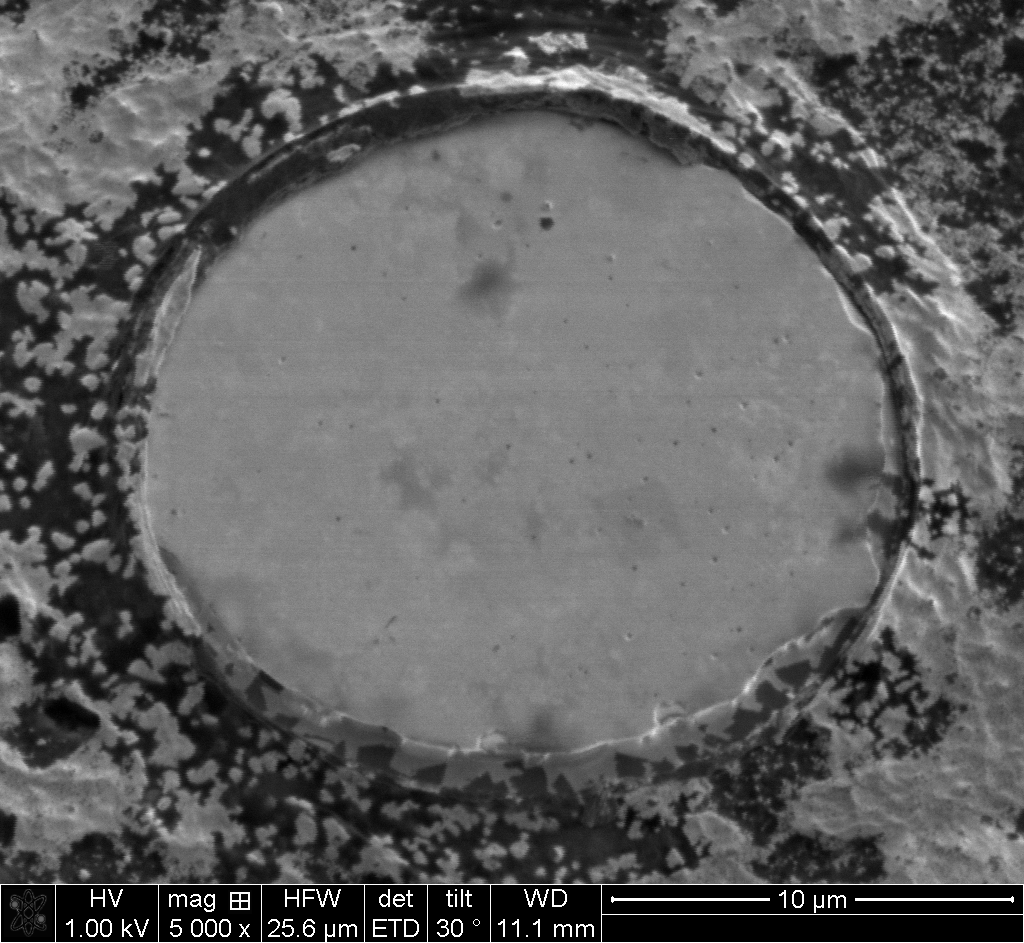
\includegraphics[trim = 0 0 0 0,  clip= true, width = \pairplotwide]{./pics/M05-13_PP_194_140926_14.png}}
			\caption{}
			\label{subfig::vcsel_sem_detail}
		\end{subfigure}
		\caption[SEM image of an array of \VCSELs]{(a) SEM image of an array of \VCSELs. The three wires are the anodes, which are connected to the top layer ($p$-contact) of the \VCSEL. Therefore, three of the \VCSEL structures can be operated. \BmFour is located in the top right whith \BmTwo to the left of it. (b) Detail SEM image of the top of \BmFour. The circular middle part is the hole in the $p$-contact through which the top DBR is visible. The smaller active diameter measures \SI{5.8}{\micro\meter} through which the laser light exits the structure is not visible in the SEM. A successful \pp operation positions a \nd hosting an \siv directly in the path of the \VCSELs laser.}
	\end{figure}

	The \VCSELs we obtained use a $n$-type DBR consisting of $50$ pairs of AlAs/Al\textsubscript{0.5}Ga\textsubscript{0.5}As mirror pairs while the $p$-type DBR is formed by $36$ Al\textsubscript{0.95}Ga\textsubscript{0.05}As/Al\textsubscript{0.5}Ga\textsubscript{0.5}As \cite{Weidenfeld2012}. The active region itself consists of $4$ GaInP quantum wells. An oxide aperture in a field node of the standing wave serves as a spatial filter for maximum modal gain by confining the current and the optical mode. The active diameter which is defined by the oxide aperture is \SI{5.8}{\micro\meter}.

	The available \VCSELs are perfect candidates for the excitation of \sivs in a hybrid integrated single photon source for several reasons. They exhibit a circular beam profile, have low divergence angel and emit linearly polarized light. Their physical size and the fact, that their output beam is perpendicular to the substrate implies that our \nds containing \nds can simply be placed on-top of the structure light-emitting region using \pp methods, see \Fref{subfig::vcsel_sem_detail}. Thus the \VCSELs output laser can be used to optically excite \sivs.

	As a first step towards using \VCSELs to excite \ccs, we characterized the behavior of \BmFour. To this end we operated it at currents of
	\SI{1.5}{\mA} and \SI{3}{\mA} and recorded the resulting lasing \wl. The emission spectra showed that the emitted \cw laser light to be around \SI{655}{\nm} in wavelength for both currents, see \Fref{subfig::vcsel_output_wavelength}. Previous research within the authors group recorded \siv intensity maxima at excitation \wls of \SI{720}{\nm} and \SI{680}{\nm} \cite{ElensMasterThesis}, aligning reasonably well with the output \wl of \BmFour.

		\begin{figure}[!htb]
			\begin{subfigure}[t]{ 0.49\linewidth}
				\centering
				\testbox{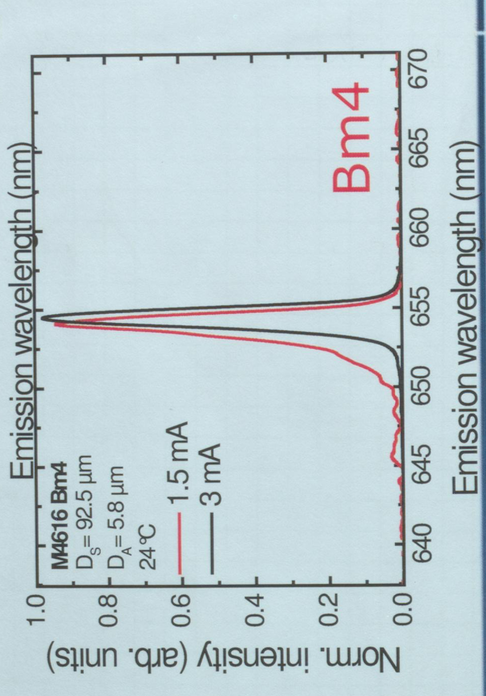
\includegraphics[trim = 0 0 0 0,  clip= true, width = \pairplotwide]{./pics/vcsel_output_wavelength.png}}
				\caption{}
				\label{subfig::vcsel_output_wavelength}
			\end{subfigure}
			\hfill
			\begin{subfigure}[t]{ 0.49\linewidth}
				\centering
				\testbox{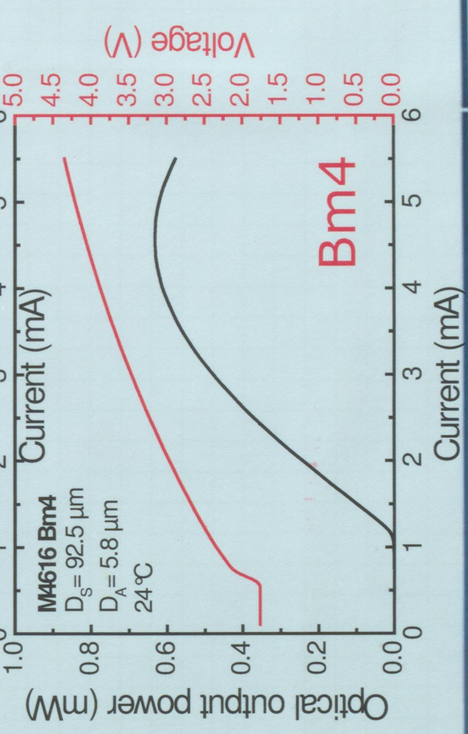
\includegraphics[trim = 0 0 0 0,  clip= true, width = \pairplotwide]{./pics/vcsel_output_power.png}}
				\caption{}
				\label{subfig::vcsel_output_power}
			\end{subfigure}
			\caption[Emission spectra and optical power of \BmFour]{(a) Emission spectrum of \BmFour at two different currents. (b) Optical output power and voltage of \BmFour in dependence of input current. Graphs extracted from a data sheet provided by \michler.}
		\end{figure}

	The optical output power of \BmFour as a function of the current applied is given in \Fref{subfig::vcsel_output_power}. In addition, the resulting voltages are shown. It can be seen that the maximum power of $\approx \SI{0.6}{\mW}$ is reached for moderate currents of $\approx \SI{4.5}{\mA}$. While the available optical powers are small comparable to using a conventional laser, low powers are sufficient for initial explorations.

	The next step consists of selecting a suitable \nd containing an \siv followed by transferring it ontop of \BmFour. To this end \nds \SI{200}{\nm} in size were grown with the \CVD method in an \ir coated \si wafer. We refer the reader to \Fref{sec::cvd} for details on the process.

	Next, using the confocal setup described in \Fref{ch::pl_setup} a \nd was identified exhibiting one dominant line at \SI{746.0}{nm} with a \lw of \SI{1.9}{nm}. Its position on the substrate was determined consecutively using a white light laser scan as described in \Fref{subsec::position}. Given the position of the \nd it was then transferred to \BmFour and placed precisely in its active, i.e.\ light-emitting region. The process of introducing an \siv to another structure is referred to as coupling.

	After successful transfer \BmFour was inserted into the confocal setup.
	Using the laser from the confocal setup we checked if the \pp process caused any modification of the spectroscopic properties of the \siv such as a decrease of count-rate or a modification of the \fl spectrum. During these checks, the \VCSEL itself was not active.

	As a first check, we scanned the \VCSEL surface in an attempt to detect the activity of the introduced \siv. \Fref{subfig::vcsel_confocal_laser_excitation_with_diamond} shows the \siv as a bright dot in the aperture of \BmFour. For comparison, a \Vcsel without coupled \siv exhibits solely background counts which is shown in \Fref{subfig::confocal_laser_excitation_without_diamond}.

	\begin{figure}[!htb]
		\begin{subfigure}[t]{ 0.49\linewidth}
			\centering
			\testbox{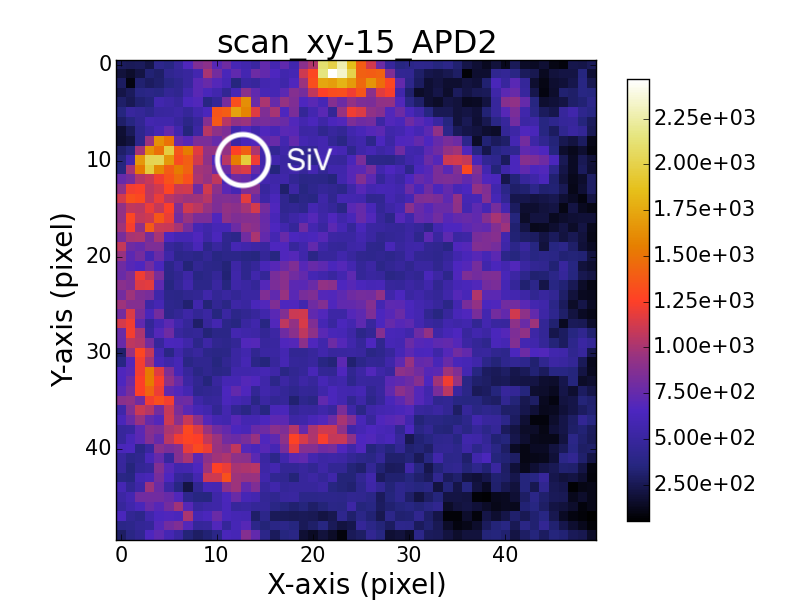
\includegraphics[trim = 0 0 0 0,  clip= true, width = \pairplotwide]{./pics/scan_xy-15_APD2_circle.png}}
			\caption{}
			\label{subfig::vcsel_confocal_laser_excitation_with_diamond}
		\end{subfigure}
		\hfill
		\begin{subfigure}[t]{ 0.49\linewidth}
			\centering
			\testbox{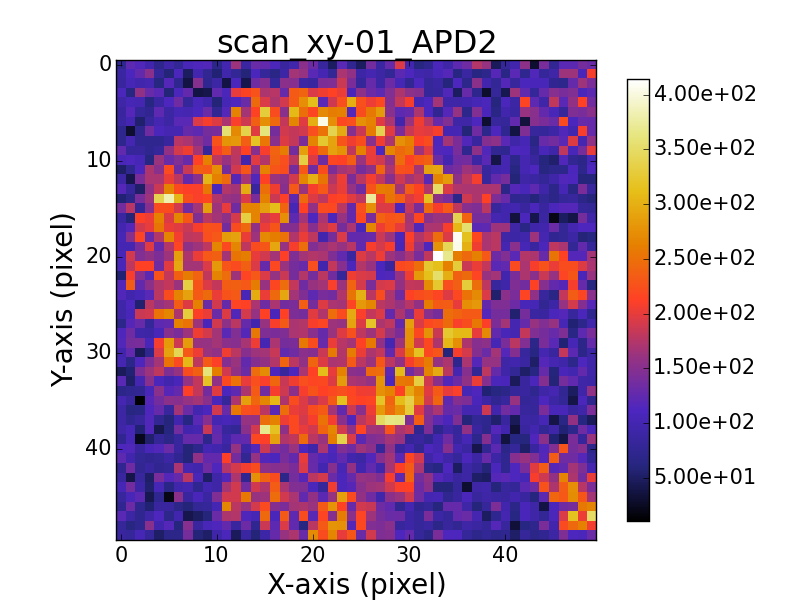
\includegraphics[trim = 0 0 0 0,  clip= true, width = \pairplotwide]{./pics/scan_xy-01_APD2.png}}
			\caption{}
			\label{subfig::confocal_laser_excitation_without_diamond}
		\end{subfigure}
		\caption[Scans of \VCSELs with and without \siv]{(a) Scan of the \BmFour with coupled \nd under excitation with the laser from the confocal setup. The big visible ring is the edge of the circular aperture in the $p$-contact of \BmFour.The bright spot in the upper left corner corresponds to the transferred \nd containing an \siv causing a spike in the count-rate. (b) Scan of the \BmTwo lacking a \nd under excitation with the laser from the confocal setup. The circular aperture in the $p$-contact exhibits a constant count-rate. Note the different scales.}
	\end{figure}

	The spectrum of the \siv in the transferred \nd was investigated before and after the \pp process. \Fref{fig::spectrum_vcsel_diamond} shows that the original spectrum before \nd transfer exhibits one dominant line at \SI{746.0}{nm}, denoted line $A$. Furthermore, two minor peaks can be seen. The lower \wl peak is denoted as line $B$. Interestingly, after the \pp process, a different picture emerges shown in \Fref{fig::spectrum_vcsel_diamond}. The once dominant line $A$ is strongly reduced. The new dominant feature is line $B$. Note that the count rate of line $B$ remained the same before and after \pp.


	\begin{figure}[!htb]
		\begin{subfigure}[t]{ 0.49\linewidth}
			\centering
			\testbox{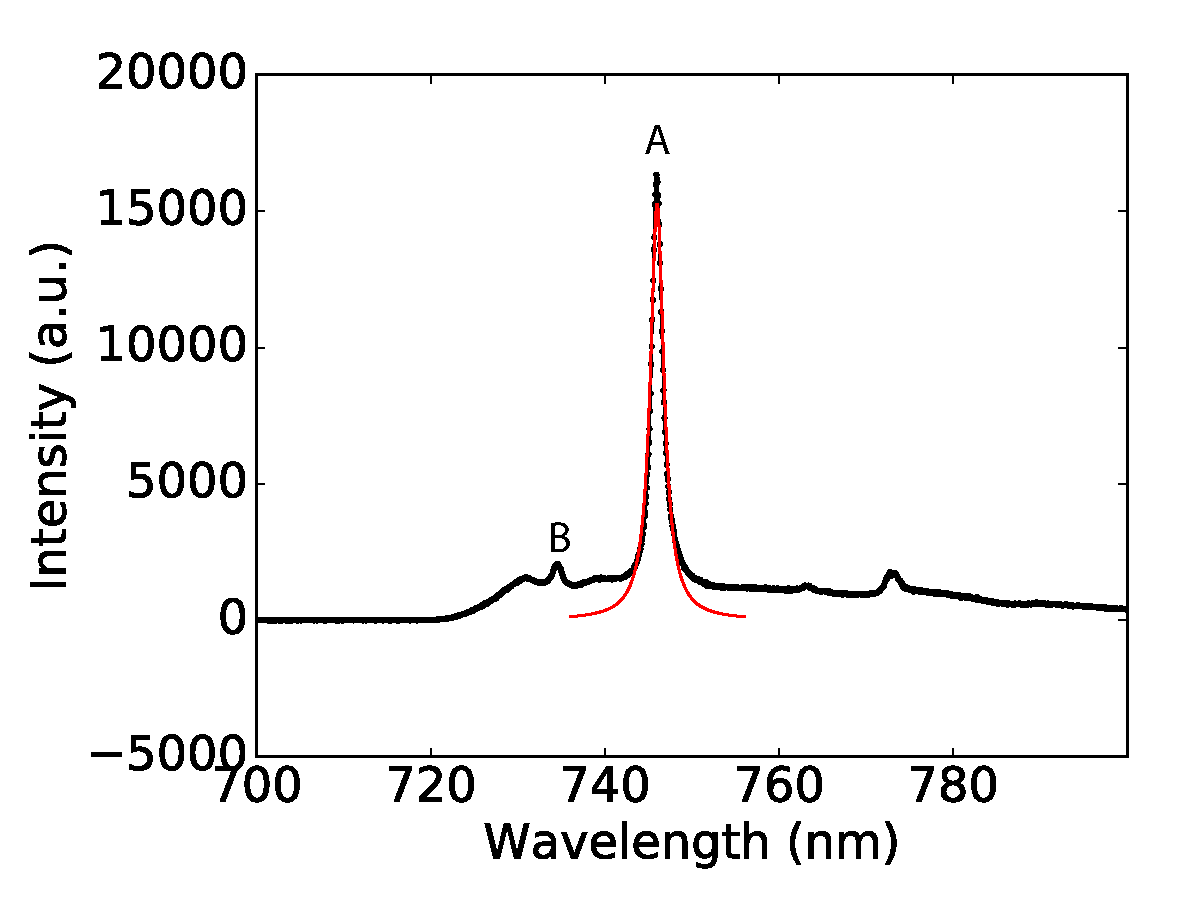
\includegraphics[trim = 0 0 0 0,  clip= true, width = \pairplotwide]{./pics/field330_scanxy06_x19y15_34uW_t30_2_fit_lines.pdf}}
			\caption{}
			\label{subfig::spectrum_diamond_for_vcsel_before_pp}
		\end{subfigure}
		\hfill
		\begin{subfigure}[t]{ 0.49\linewidth}
			\centering
			\testbox{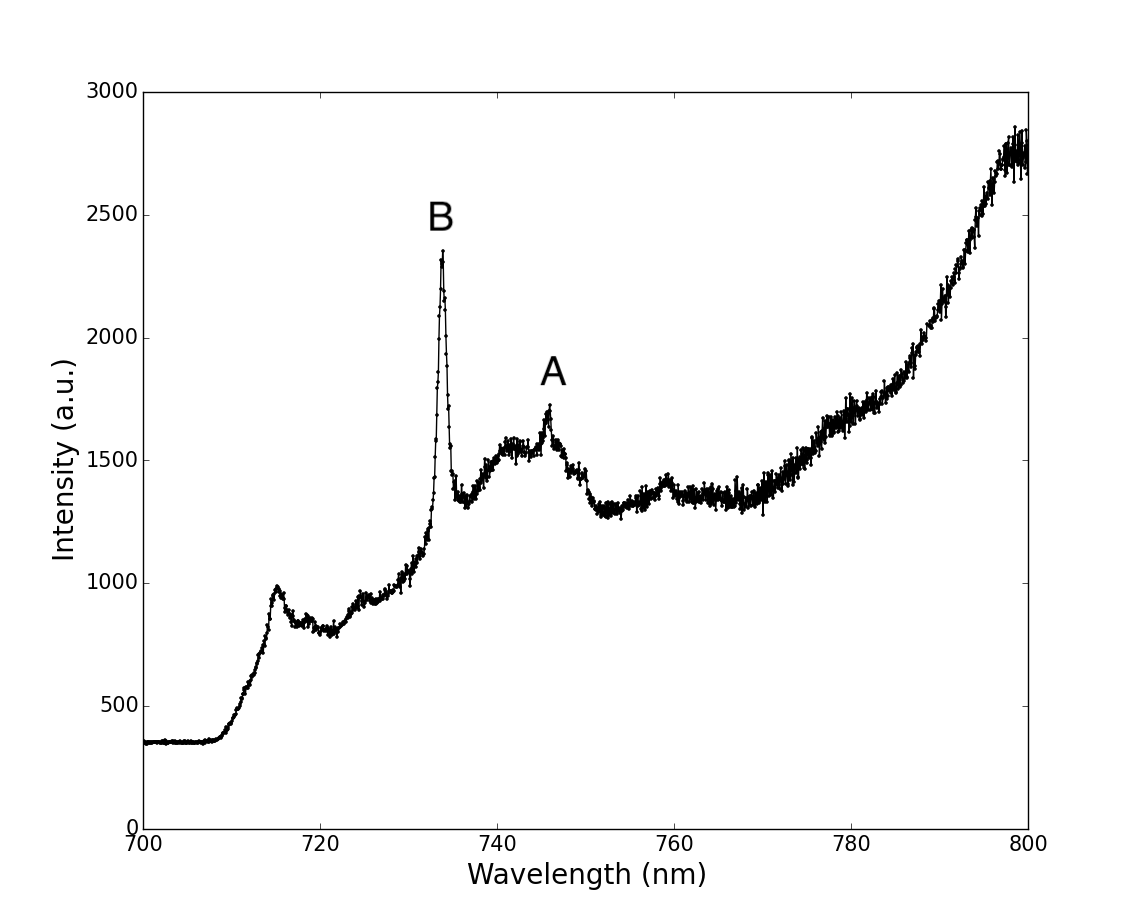
\includegraphics[trim = 0 0 0 0,  clip= true, width = \pairplotwide]{./pics/spe_scan_xy-25_300uW_t60_700-800nm_lines.png}}
			\caption{}
			\label{subfig::spectrum_vcsel_confocal_excitation_with_diamond}
		\end{subfigure}
		\caption[\Siv properties before and after \pp]{(a) Spectrum of the preselected diamond for transfer onto \BmFour before \pp. The strong line denoted $A$ exhibits a \cwl of \SI{746.0}{nm} and a \lw of \SI{1.9}{nm}. Line $B$ exhibits a \cwl of \SI{734.5}{\nm} and a \lw of \SI{3.8}{\nm}. (b) Spectrum of the same \siv after \pp, excited with the same laser as before. While Line $A$ is almost gone, line $B$ still exists seemingly unchanged and has become the predominant line of the spectrum. We remark that due to material restrictions, different long-pass filters were used for the two measurements. Measurement (a) was performed with a \SI{720}{nm} long-pass filter, measurement (b) with a \SI{710}{nm} longpass filter.}
		\label{fig::spectrum_vcsel_diamond}
	\end{figure}

	The observed reduction of the intensity of line $A$ is difficult to explain. One cause could be damage to the \cc due to the electron radiation it was exposed to during the \pp process. This is supported by previous research in this authors group recording reduced \fl intensities after \ccs were exposed to electron radiation \cite{MeyerBaccThesis}. However, the fact that line $B$ remains virtually the same before and after \pp is curious, raising the question whether damage alone is sufficient to explain the observed effect. As it stands, the question remains open and is thus subject to further investigation.

	With line $B$ as remaining dominant line we then operated \BmFour at \SI{1.84}{mA} and \SI{3.3}{V}, turning off the laser of the confocal setup.
	Thus \siv excitation is due to the output laser of \BmFour.

	For comparison, we scanned both the surface of \BmFour including a \nd as well as \BmTwo without a \nd. A bandpass filter allowing light between \SIrange{730}{750}{\nm} to pass was used.
	This filter window suppresses the \VCSEL laser line at \SI{655}{\nm} while leaving the \siv emission nearly unchanged. The results of the two scans are given in \Fref{fig::vcsel_excitation}, where the bright areas correspond to the circular \VCSEL output regions. It can be seen that no difference in brightness can be established between a \VCSEL with and without a \nd containing a \siv.

		\begin{figure}[!htb]
			\begin{subfigure}[t]{ 0.49\linewidth}
				\centering
				\testbox{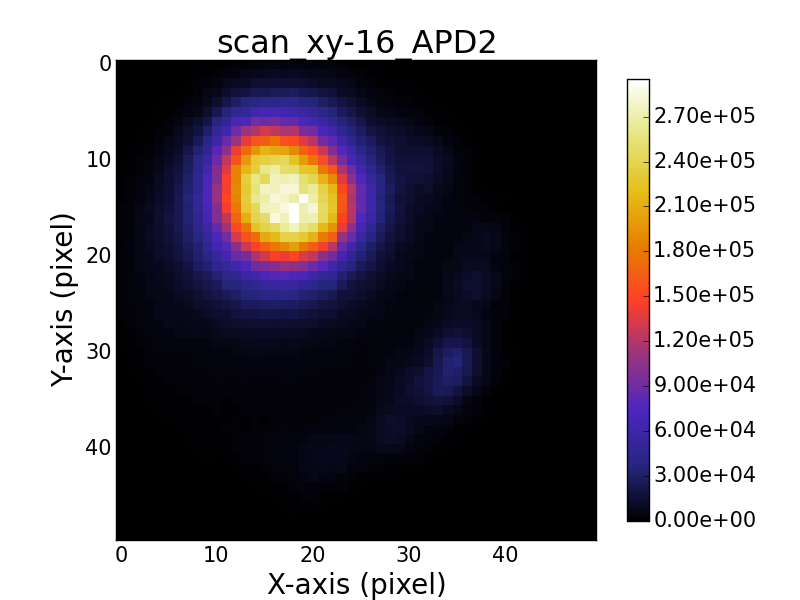
\includegraphics[trim = 0 0 0 0,  clip= true, width = \pairplotwide]{./pics/scan_xy-16_APD2.png}}
				\caption{}
				\label{subfig::vcsel_excitation_with_diamond}
			\end{subfigure}
			\hfill
			\begin{subfigure}[t]{ 0.49\linewidth}
				\centering
				\testbox{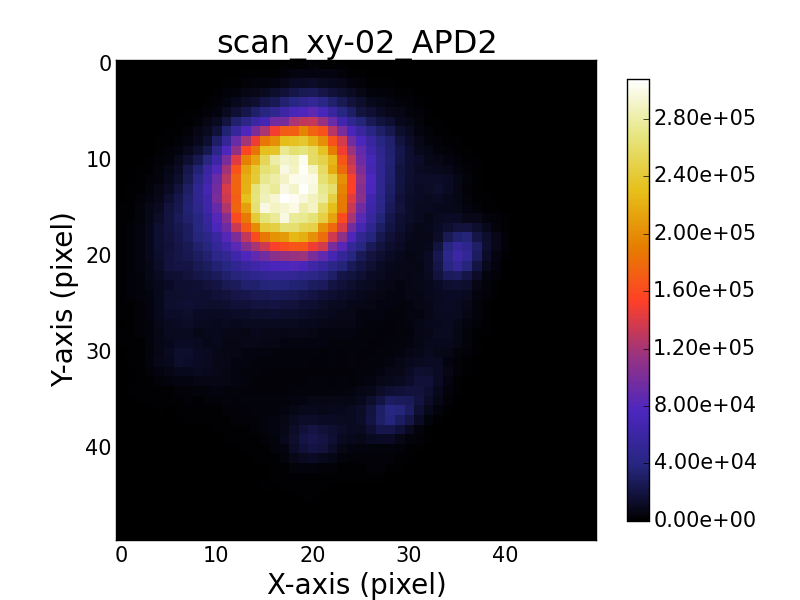
\includegraphics[trim = 0 0 0 0,  clip= true, width = \pairplotwide]{./pics/scan_xy-02_APD2.png}}
				\caption{}
				\label{subfig::vcsel_excitation_without_diamond}
			\end{subfigure}
			\caption[Comparison of intensities between \BmFour and \BmTwo]{(a) Scan of the laser light stemming from \BmFour and the \fl from the \siv in the filter window \SIrange{730}{750}{nm}. (b) Scan of the laser light stemming from \BmTwo without a coupled \siv. The outcome of the two scans is almost identical.}
			\label{fig::vcsel_excitation}
		\end{figure}


		To further investigate we conduct spectroscopic measurements. Since the position of the \nd in \BmFour is known, we measure the spectrum of light originating from this position. A second spectrum is obtained from \BmTwo measuring the corresponding position without a \nd present. \Fref{fig::vcsel_spectra} reports the results. Again no meaningful difference between the two \VCSELs can be established. The lack of any distinct lines in the spectrum taken for \BmFour{} which can be attributed to \siv emission is striking.

			\begin{figure}[!htb]
				\begin{subfigure}[t]{ 0.49\linewidth}
					\centering
					\testbox{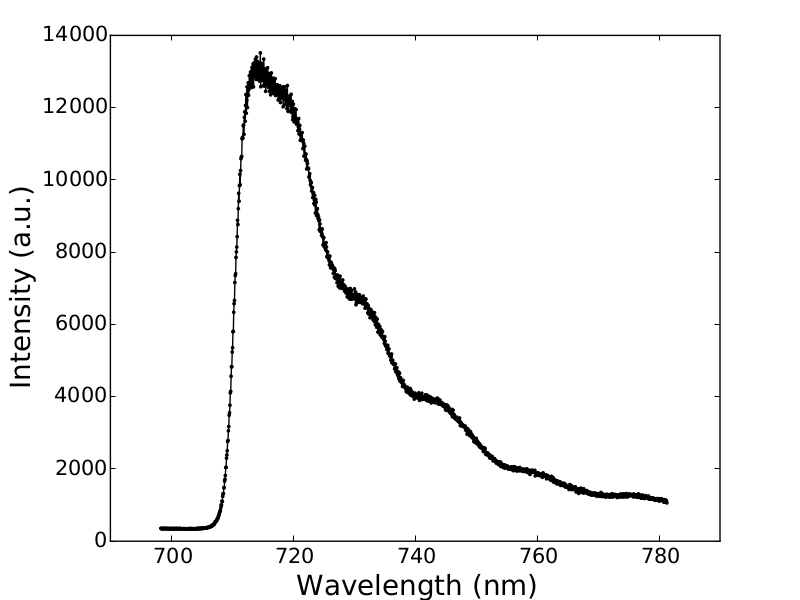
\includegraphics[trim = 0 0 0 0,  clip= true, width = \pairplotwide]{./pics/spe_VCSEL_excitation_diamond_5.png}}
					\caption{}
					\label{subfig::spectrum_vcsel_excitation_with_diamond}
				\end{subfigure}
				\hfill
				\begin{subfigure}[t]{ 0.49\linewidth}
					\centering
					\testbox{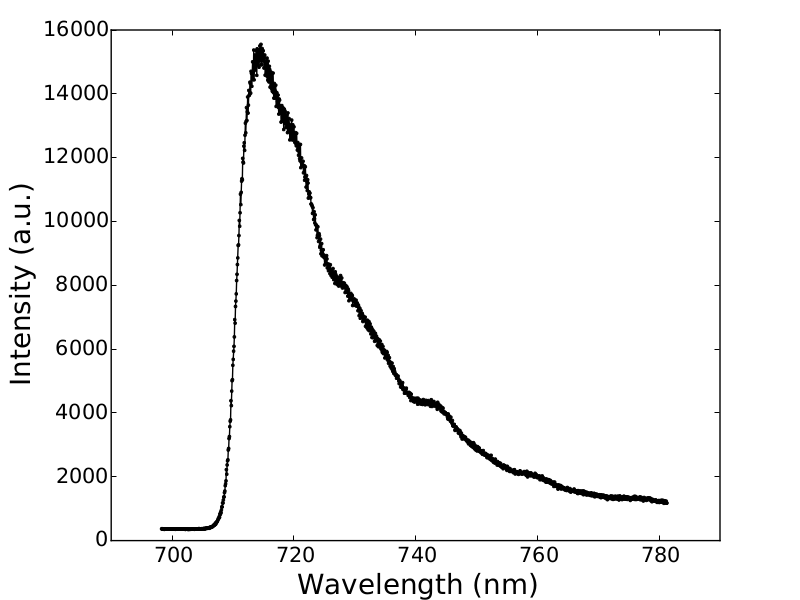
\includegraphics[trim = 0 0 0 0,  clip= true, width = \pairplotwide]{./pics/spe_VCSEL_excitation_diamond_Bm2.png}}
					\caption{}
					\label{subfig::spectrum_vcsel_excitation_without_diamond}
				\end{subfigure}
				\caption[Comparison of spectra between \BmFour and \BmTwo]{(a) Recorded Spectrum of the \siv in the transferred \nd coupled to \BmFour during VCSEL operation. No distinct \siv lines are visible. (b) Recorded spectrum of \BmTwo.}
				\label{fig::vcsel_spectra}
			\end{figure}

		To explain the observation, the following considerations are reasonable: The \siv is excited by the \VCSELs laser and thus emitting single photons which are passing through the filter window. The same is true for photons stemming from \VCSEL \sb emission. Given that the emission from the \sb of \BmFour dwarfs the single photon emission of its \siv, the obtained results are reasonable.
		To confirm we examine the reflectivity of the DBR of \BmFour. \Fref{fig::dbr_vcsel} illustrates that the DBR exhibits imperfect reflexivity in the wavelength region relevant for \siv emission. As a result, relevant \sb emissions of \BmFour are not sufficiently suppressed to allow for \siv emission to be detected. This in turn means that our initial attempt to realize a hybrid-integrated \sps by coupling an \siv to a \VCSELs is thwarted by large \sb emissions of the latter.

		\begin{figure}[!htb]
			\centering
			\testbox{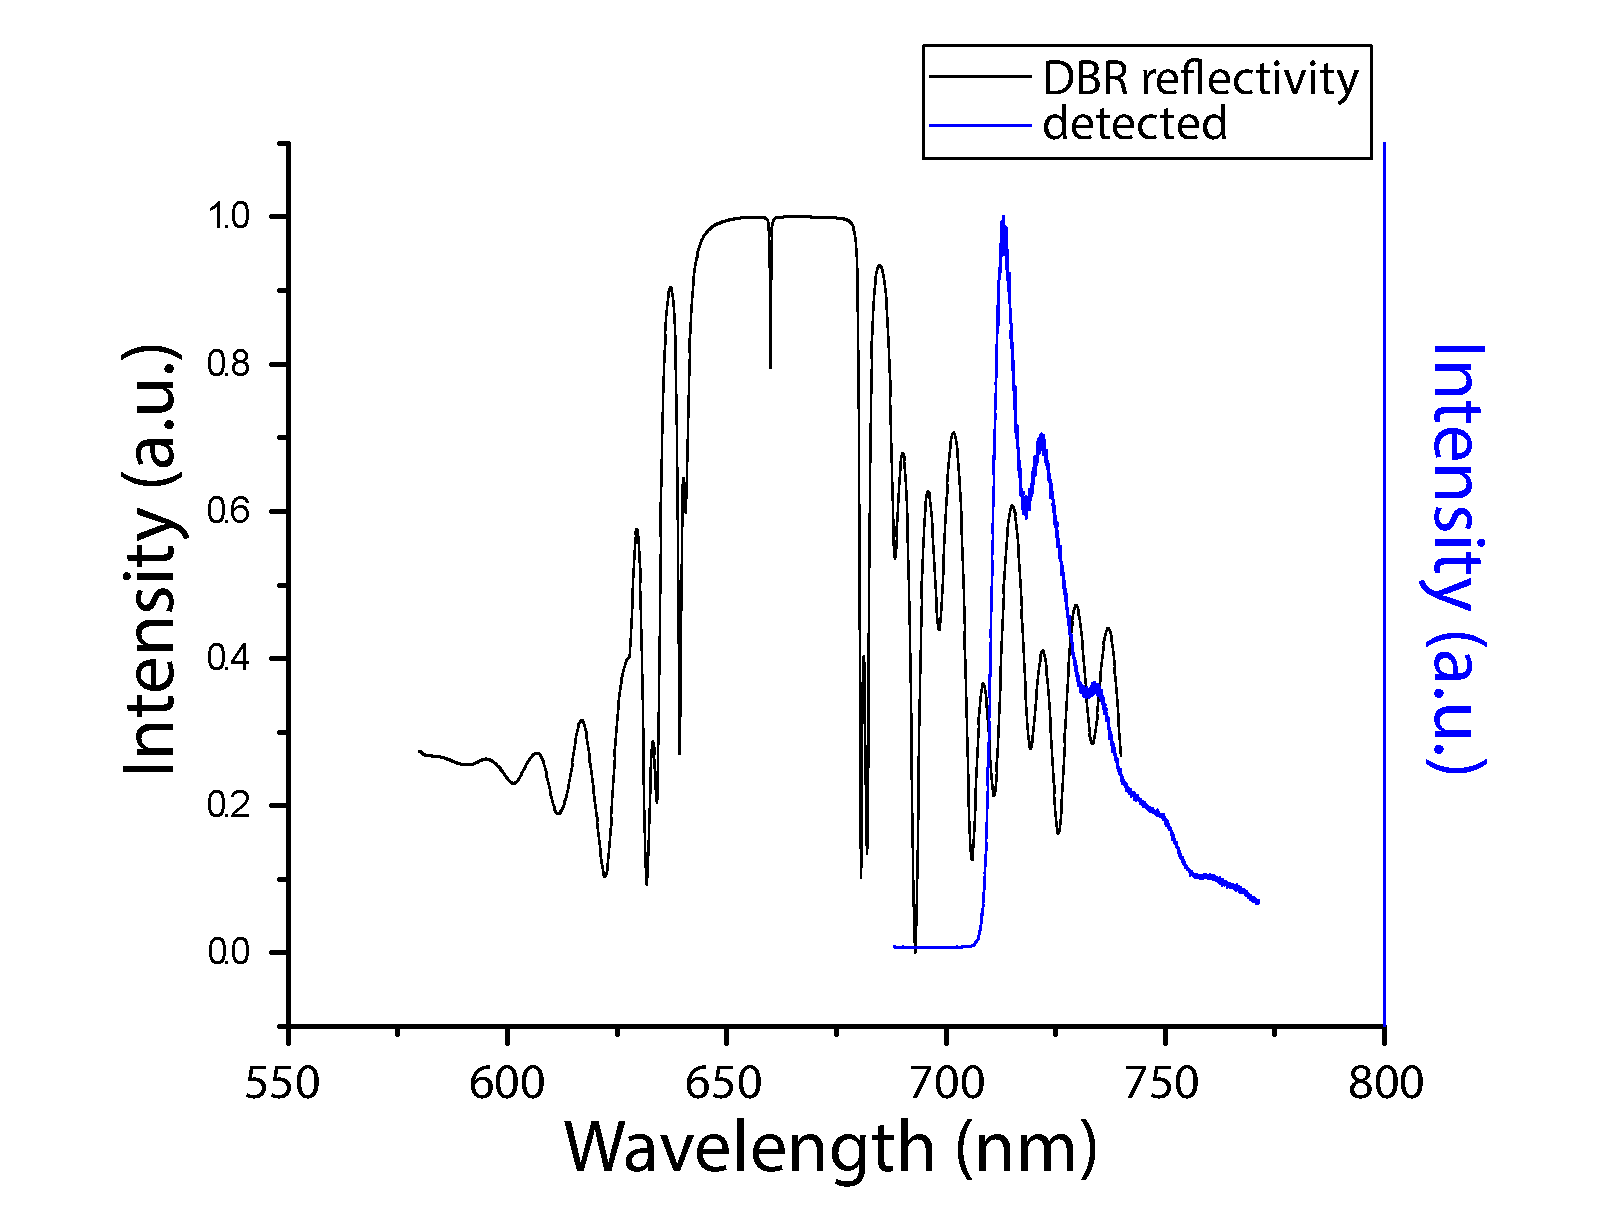
\includegraphics[trim = 0 0 0 0,  clip= true, width = 0.5\textwidth]{./pics/dbr_VCSEL_only_blue.pdf}}
			\caption[Reflectivity of \BmFour]{Reflectivity of the \dbr (DBR) of \BmFour \cite{Weidenfeld2012}, and a spectrum of the \siv measured during \VCSEL excitation for comparison. The reflectivity of the DBR and the VCSEL emission spectra are depicted with different scales. The shape of the measurement of the \siv during \VCSEL operation is reminiscent of the shape of the DBR reflectivity. The spectrum of the \siv is not visible. As the emission from the \siv is small compared to the intensity of the laser \sb in the same wavelength regime, the \sivs emission is not.}
			\label{fig::dbr_vcsel}
		\end{figure}

		Despite a failed first attempt, a clear direction for further improvement was identified, i.e.\ focusing on ways to reduce \VCSEL \sb emission in the relevant \siv emission regime. A promising approach to suppress the \sb is to add a gold layer on top of the \VCSEL acting as an additional mirror. While films of gold have a transmittance maximum at \SI{500}{nm}, the transmittance minimum depends on the film's thickness \cite{Axelevitch2012}. Thus a gold layer could in principle be used to suppress the \VCSEL \sb in the \siv emission regime. Provided such a layer can be engineered and is effective, one may expect \siv emission to be recovered. Efforts in this direction are a required next step towards the realization of hybrid-integrated \spss based on \sivs coupled to \VCSELs.
